\documentclass[12pt]{article}
\usepackage{amsmath,amsfonts,amsthm,amssymb}
\usepackage{setspace}
\usepackage{fancyhdr}
\usepackage{lastpage}
\usepackage{extramarks}
\usepackage[ruled,vlined]{algorithm2e}
\usepackage{chngpage}
\usepackage{soul,color}
\usepackage[final]{graphicx}
\usepackage{float, wrapfig}
\usepackage{listings}
\usepackage{enumitem}
\usepackage{indentfirst}
\usepackage{multicol}


\newcommand{\Class}{\normalsize CS 370: Introduction to Computational Geometry}

\newcommand{\Title}{Assignment 2}
\newcommand{\StudentName}{Brady Zhou}
\newcommand{\StudentClass}{50705}
\newcommand{\StudentNumber}{bz2459}

\topmargin=-0.45in
\evensidemargin=0in
\oddsidemargin=0in
\textwidth=6.5in
\textheight=9.0in
\headsep=0.25in

\setlength{\parindent}{5ex}

\pagestyle{fancy}
\lhead{\StudentName}
\rhead{\firstxmark}
\lfoot{\lastxmark}
\cfoot{}
\rfoot{Page\ \thepage\ of\ \protect\pageref{LastPage}}
\renewcommand\headrulewidth{0.4pt}
\renewcommand\footrulewidth{0.4pt}

\title{\textmd{\bf \Class\\}}
\author{\small \normalfont{Advisor: Chandrajit Bajaj} \\
\small \normalfont{\StudentName}}
\date{} 

\begin{document}

\maketitle \thispagestyle{empty}

\noindent {\large \textbf{Abstract}} \newline \\
\indent The goal of this independent study course is to explore the fundamentals of computational geometry. In this semester long course, the topics covered will include turn orientation, convex hull, minkowski sum, triangulations, delanauy triangulations, voronoi diagrams, and more topics not decided yet. Professor Bajaj will advise by suggesting topics and papers to explore. The tools used will include \textbf{CGAL}, a computational geometry library in C++, and \textbf{matplotlib}, a Python library used for charting.
\newpage

\begin{multicols}{2}
\subsection{Turn Orientation}

\indent A key recurring theme in computation is the problem of floating point error. A common tool in the geometry toolbox is the idea of \textbf{turn orientation}, that is, whether a set of three points makes a clockwise (right), or counter-clockwise (left) turn. In a naive implementation of determining orientation of a turn, the angle of the line formed is calculated using some form of division and arcos. This can lead to loss of precision due to floating point numbers. \newline
\indent A better way to deal with line orientation is to take the determinant of the three points and if the determinant is larger than some $\epsilon$, the points make a clockwise turn. If the determinant falls within $-\epsilon$ to $\epsilon$, we say the points are colinear, and if the determinant is smaller than $\epsilon$, the points make a counter-clockwise turn. The benefits of using this implementation is that accurascy is more robust as it does not use division. \newline \\
\centerline{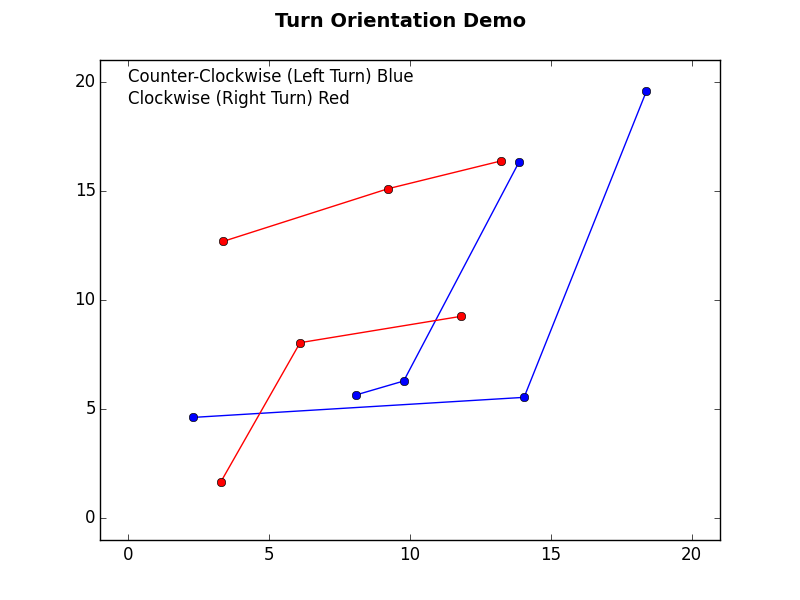
\includegraphics[scale=.4]{turn_orientation.png}}

\subsection{Convex Hull}
\indent With just a one tool in our geometry toolbox, we can solve a fundamental problem of computational geometry - computing the \textbf{convex hull} of a set of points $X$. A convex hull is defined as the minimal subset of points that envelop $X$, or more formally, the intersection of all convex sets containing all $X$. There are well many well-known algorithms, but the one of interest is the Graham Scan, which was published in 1972. \newline \\
\centerline{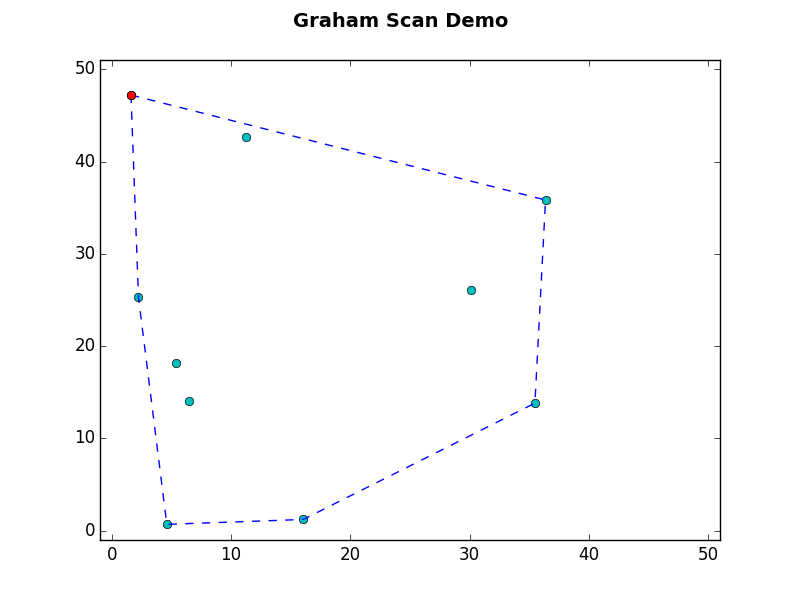
\includegraphics[scale=0.4]{graham_scan.png}}
\indent The algorithm works by splitting the problem into two problems - finding the upper hull and then the lower hull. On a high level, to find the upper hull, we iterate over the points from left to right and have a result set $R$ of points in upper hull. We keep appending points onto our result set and then check to see if the last points make a right turn. If they do not, we know the middle point is not a part of our final result set and we delete the middle point from the result set. We continue this until there are less than 3 points to make a turn, or the last three points do make a right turn. When the algorithm reaches the rightmost point, it terminates and returns the upper hull. The lower hull is computed using the same concept, but all the points in the lower hull will make left turns. \newline
\indent If we assume the list of points $P$ is sorted in increasing x order, the runtime algorithm is $O(n)$ where $n = |P|$, as the algorithm will iterate over the list once for each hull - upper and lower. Otherwise, if the list of points is not sorted, we will have to do so and that will be the dominating time complexity of $O(n\ log\ n)$.  The psuedocode for the algorithm is as follows. \newline \\
\textbf{Algorithm} UpperConvexHull($P$) \newline 
\emph{Input:} A set $P$ of points to enclose. \newline
\emph{Output:} A set $R$, which is a subset of $P$. \newline
Sort $P$ by x-coordinate. \newline
Add $p_1, p_2$ to $R$. \newline
\textbf{for} $i \leftarrow 3$ \textbf{to} $n$ \newline
\indent Add $p_i$ to $R$. \newline
\indent \textbf{while} $r_{n-2},\ r_{n-1},\ r_n$ do not make a right turn \newline
\indent \indent Remove $r_{n-1}$ from $R$. \newline
\textbf{return} $R$. \newline \\
With this algorithm, we have to be careful in certain cases. In the case we have a triple of colinear points on the hull, our algorithm should not include the middle point as the convex hull is defined as the minimal set of points. However, we can fix this relatively easy by ensuring our function that checks right turns returns false if the points are colinear, that is, if the determinant is zero or less.
\subsection{Minkowski Sum}
\indent 

\subsection{Triangulations}
\indent blah blah

\end{multicols}
\end{document}
